\chapter{Localized Questions in Medical Visual Question Answering}
\label{appendix:locvqa}

\begin{table}[!t]
\ra{1.2}
\begin{center}
\begin{tabular}{p{0.1cm}p{0.2\linewidth}p{0.01cm}LKLKL}
\toprule
{} &\multirow{2}{*}{Instrument}  & \multicolumn{6}{c}{Method} \\
\cmidrule{3-8} 
&         && Ignore mask & Region in Text & Crop Region & Draw Region & \ours  \\ \midrule
&Eye retractors    && \makecell[tc]{0.500 \\ $\pm$0}              & \makecell[tc]{0.822 \\ $\pm$0.005}                     & \makecell[tc]{0.882 \\ $\pm$0.002}            & \makecell[tc]{\textbf{0.913} \\$\pm$\textbf{0.002}}                 & \makecell[tc]{0.912 \\ $\pm$0.004}                        \\ 
& Rycroft cannula &&   \makecell[tc]{0.500 \\ $\pm$0}                  &   \makecell[tc]{0.728\\$\pm$0.025}                        &     \makecell[tc]{0.847\\$\pm$0.002}          &        \makecell[tc]{0.910\\$\pm$0.002}       & \makecell[tc]{\textbf{0.912}\\$\pm$\textbf{0.001}}                   \\ 
&Viter. handpiece    && \makecell[tc]{0.500 \\ $\pm$0}               & \makecell[tc]{0.805 \\$\pm$0.024}                     & \makecell[tc]{\textbf{0.960}\\$\pm$\textbf{0.006}}         & \makecell[tc]{0.953\\$\pm$0.005}              & \makecell[tc]{0.881 \\$\pm$0.010}                     \\ 
&Secondary knife &&      \makecell[tc]{0.500 \\ $\pm$0}           &   \makecell[tc]{0.751\\$\pm$0.013}       &   \makecell[tc]{0.822\\$\pm$0.013}      &  \makecell[tc]{0.828\\$\pm$0.011}       &  \makecell[tc]{\textbf{0.830}\\$\pm$\textbf{0.007}}                   \\ 

&Suture needle          && \makecell[tc]{0.500 \\ $\pm$0}                & \makecell[tc]{0.825 \\$\pm$0.019}                     & \makecell[tc]{\textbf{0.889} \\$\pm$\textbf{0.004}}         & \makecell[tc]{0.851 \\$\pm$0.014}              & \makecell[tc]{0. 848\\$\pm$0.018}    \\

&Micro-manipulator&&       \makecell[tc]{0.500 \\ $\pm$0}             &   \makecell[tc]{0.645\\$\pm$0.032}       &   \makecell[tc]{0.846\\$\pm$0.003}      &  \makecell[tc]{0.877\\$\pm$0.007}       &  \makecell[tc]{\textbf{0.889}\\$\pm$\textbf{0.004}}                   \\ 

&Bonn forceps&&       \makecell[tc]{0.500 \\ $\pm$0}              &   \makecell[tc]{0.846\\$\pm$0.020}       &   \makecell[tc]{0.908\\$\pm$0.008}      &  \makecell[tc]{0.897\\$\pm$0.012}       &  \makecell[tc]{\textbf{0.909}\\$\pm$\textbf{0.004}}                   \\ 

&Visco. cannula&&       \makecell[tc]{0.500 \\ $\pm$0}              &   \makecell[tc]{0.879\\$\pm$0.013}       &   \makecell[tc]{\textbf{0.954}\\$\pm$\textbf{0.002}}      &  \makecell[tc]{0.946\\$\pm$0.003}       &  \makecell[tc]{0.937\\$\pm$0.003}                   \\

&Cap. forceps&&       \makecell[tc]{0.500 \\ $\pm$0}              &   \makecell[tc]{0.804\\$\pm$0.039}       &   \makecell[tc]{0.905\\$\pm$0.010}      &  \makecell[tc]{\textbf{0.932}\\$\pm$\textbf{0.018}}       &  \makecell[tc]{0.908\\$\pm$0.010}                   \\

&Phaco. handpiece&&      \makecell[tc]{0.500 \\ $\pm$0}              &   \makecell[tc]{0.717\\$\pm$0.037}       &   \makecell[tc]{0.900\\$\pm$0.008}      &  \makecell[tc]{0.920\\$\pm$0.003}       &  \makecell[tc]{\textbf{0.952}\\$\pm$\textbf{0.003}}                   \\

&Charleux cannula&&       \makecell[tc]{0.500 \\ $\pm$0}              &   \makecell[tc]{0.841\\$\pm$0.044}       &   \makecell[tc]{0.826\\$\pm$0.029}      &  \makecell[tc]{0.915\\$\pm$0.016}       &  \makecell[tc]{\textbf{0.925}\\$\pm$\textbf{0.016}}                   \\

&Lens injector&&      \makecell[tc]{0.500 \\ $\pm$0}            &   \makecell[tc]{0.773\\$\pm$0.006}       &   \makecell[tc]{\textbf{0.941}\\$\pm$\textbf{0.003}}      &  \makecell[tc]{0.927\\$\pm$0.007}       &  \makecell[tc]{0.917\\$\pm$0.007}                   \\

&Cap. cystotome&&       \makecell[tc]{0.500 \\ $\pm$0}              &   \makecell[tc]{0.789\\$\pm$0.009}       &   \makecell[tc]{0.938\\$\pm$0.006}      &  \makecell[tc]{0.934\\$\pm$0.002}       &  \makecell[tc]{\textbf{0.953}\\$\pm$\textbf{0.001}}                   \\

&Primary knife&&      \makecell[tc]{0.500 \\ $\pm$0}              &   \makecell[tc]{0.846\\$\pm$0.011}       &   \makecell[tc]{\textbf{0.954}\\$\pm$\textbf{0.003}}      &  \makecell[tc]{0.926\\$\pm$0.008}       &  \makecell[tc]{0.941\\$\pm$0.004}                   \\

&Hydro. cannula&&       \makecell[tc]{0.500 \\ $\pm$0}               &   \makecell[tc]{0.865\\$\pm$0.006}       &   \makecell[tc]{0.939\\$\pm$0.004}          &  \makecell[tc]{\textbf{0.945}\\$\pm$\textbf{0.006}}    & \makecell[tc]{0.940\\$\pm$0.004}               \\

&A/I handpiece&&      \makecell[tc]{0.500 \\ $\pm$0}            &   \makecell[tc]{0.877\\$\pm$0.021}       &   \makecell[tc]{0.935\\$\pm$0.006}      &  \makecell[tc]{0.906\\$\pm$0.004}       &  \makecell[tc]{\textbf{0.938}\\$\pm$\textbf{0.001}}        \\           
\bottomrule
\end{tabular}
\end{center}
\caption{Average test AUC for different methods on INSEGCAT-VQA. 
}
\label{tab:results_insegcat_object}
\end{table}



\begin{figure}
\begin{center}
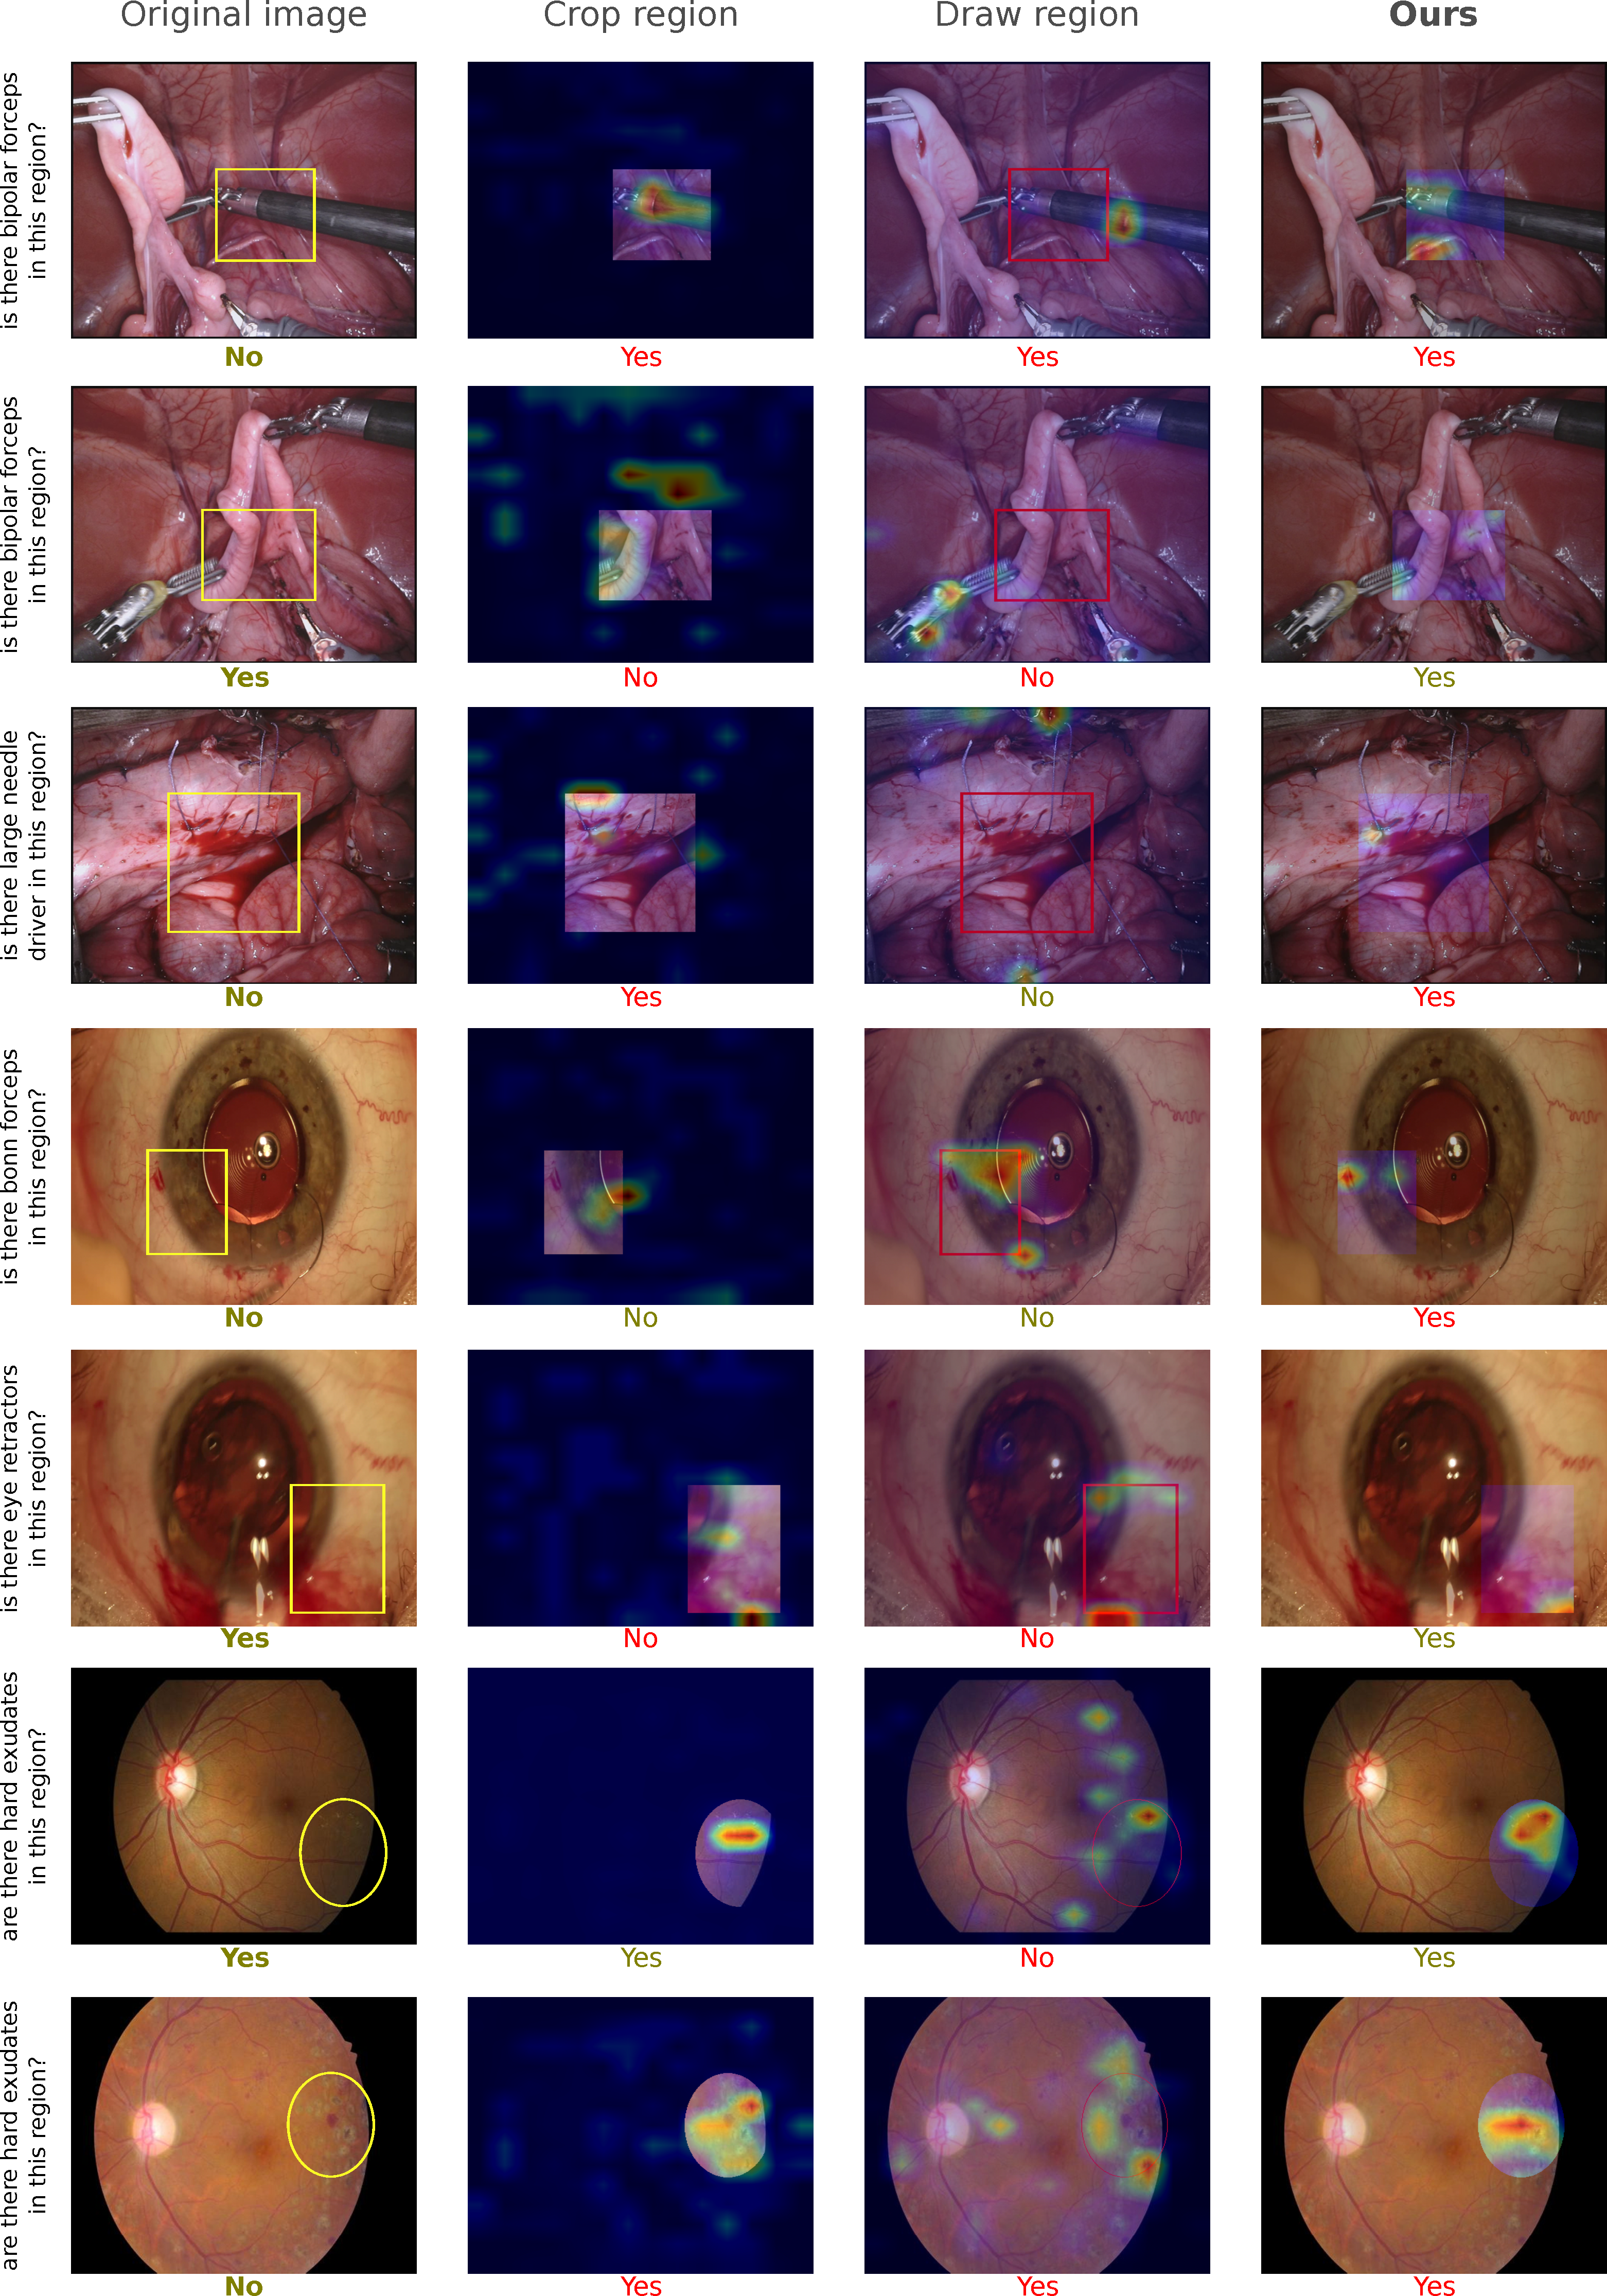
\includegraphics[width=\textwidth]{Figures/Part1_LocVQA/01_locatt/examples_att_supp.pdf}
\caption{Additional qualitative examples from the RIS-VQA (rows 1-3), INSEGCAT-VQA (rows 4-5) and DME-VQA (last two rows) datasets. The first column shows the image, the region, and the ground truth answer. Other columns show the overlaid attention maps and the answers produced by each model. Wrong answers are shown in red.}
\label{fig:examples_supp1}
\end{center}
\end{figure}



